\documentclass[journal, a4paper]{IEEEtran}

\usepackage{booktabs}
\usepackage{subcaption}
\usepackage{hyperref} % links
%\usepackage{mathabx} % asterisk
%\usepackage{cite}      % Written by Donald Arseneau
                        % V1.6 and later of IEEEtran pre-defines the format
                        % of the cite.sty package \cite{} output to follow
                        % that of IEEE. Loading the cite package will
                        % result in citation numbers being automatically
                        % sorted and properly "ranged". i.e.,
                        % [1], [9], [2], [7], [5], [6]
                        % (without using cite.sty)
                        % will become:
                        % [1], [2], [5]--[7], [9] (using cite.sty)
                        % cite.sty's \cite will automatically add leading
                        % space, if needed. Use cite.sty's noadjust option
                        % (cite.sty V3.8 and later) if you want to turn this
                        % off. cite.sty is already installed on most LaTeX
                        % systems. The latest version can be obtained at:
                        % http://www.ctan.org/tex-archive/macros/latex/contrib/supported/cite/

\usepackage{graphicx}   % Written by David Carlisle and Sebastian Rahtz
                        % Required if you want graphics, photos, etc.
                        % graphicx.sty is already installed on most LaTeX
                        % systems. The latest version and documentation can
                        % be obtained at:
                        % http://www.ctan.org/tex-archive/macros/latex/required/graphics/
                        % Another good source of documentation is "Using
                        % Imported Graphics in LaTeX2e" by Keith Reckdahl
                        % which can be found as esplatex.ps and epslatex.pdf
                        % at: http://www.ctan.org/tex-archive/info/

%\usepackage{psfrag}    % Written by Craig Barratt, Michael C. Grant,
                        % and David Carlisle
                        % This package allows you to substitute LaTeX
                        % commands for text in imported EPS graphic files.
                        % In this way, LaTeX symbols can be placed into
                        % graphics that have been generated by other
                        % applications. You must use latex->dvips->ps2pdf
                        % workflow (not direct pdf output from pdflatex) if
                        % you wish to use this capability because it works
                        % via some PostScript tricks. Alternatively, the
                        % graphics could be processed as separate files via
                        % psfrag and dvips, then converted to PDF for
                        % inclusion in the main file which uses pdflatex.
                        % Docs are in "The PSfrag System" by Michael C. Grant
                        % and David Carlisle. There is also some information
                        % about using psfrag in "Using Imported Graphics in
                        % LaTeX2e" by Keith Reckdahl which documents the
                        % graphicx package (see above). The psfrag package
                        % and documentation can be obtained at:
                        % http://www.ctan.org/tex-archive/macros/latex/contrib/supported/psfrag/

%\usepackage{subfigure} % Written by Steven Douglas Cochran
                        % This package makes it easy to put subfigures
                        % in your figures. i.e., "figure 1a and 1b"
                        % Docs are in "Using Imported Graphics in LaTeX2e"
                        % by Keith Reckdahl which also documents the graphicx
                        % package (see above). subfigure.sty is already
                        % installed on most LaTeX systems. The latest version
                        % and documentation can be obtained at:
                        % http://www.ctan.org/tex-archive/macros/latex/contrib/supported/subfigure/

\usepackage{url}        % Written by Donald Arseneau
                        % Provides better support for handling and breaking
                        % URLs. url.sty is already installed on most LaTeX
                        % systems. The latest version can be obtained at:
                        % http://www.ctan.org/tex-archive/macros/latex/contrib/other/misc/
                        % Read the url.sty source comments for usage information.

%\usepackage{stfloats}  % Written by Sigitas Tolusis
                        % Gives LaTeX2e the ability to do double column
                        % floats at the bottom of the page as well as the top.
                        % (e.g., "\begin{figure*}[!b]" is not normally
                        % possible in LaTeX2e). This is an invasive package
                        % which rewrites many portions of the LaTeX2e output
                        % routines. It may not work with other packages that
                        % modify the LaTeX2e output routine and/or with other
                        % versions of LaTeX. The latest version and
                        % documentation can be obtained at:
                        % http://www.ctan.org/tex-archive/macros/latex/contrib/supported/sttools/
                        % Documentation is contained in the stfloats.sty
                        % comments as well as in the presfull.pdf file.
                        % Do not use the stfloats baselinefloat ability as
                        % IEEE does not allow \baselineskip to stretch.
                        % Authors submitting work to the IEEE should note
                        % that IEEE rarely uses double column equations and
                        % that authors should try to avoid such use.
                        % Do not be tempted to use the cuted.sty or
                        % midfloat.sty package (by the same author) as IEEE
                        % does not format its papers in such ways.

\usepackage{amsmath}    % From the American Mathematical Society
                        % A popular package that provides many helpful commands
                        % for dealing with mathematics. Note that the AMSmath
                        % package sets \interdisplaylinepenalty to 10000 thus
                        % preventing page breaks from occurring within multiline
                        % equations. Use:
%\interdisplaylinepenalty=2500
                        % after loading amsmath to restore such page breaks
                        % as IEEEtran.cls normally does. amsmath.sty is already
                        % installed on most LaTeX systems. The latest version
                        % and documentation can be obtained at:
                        % http://www.ctan.org/tex-archive/macros/latex/required/amslatex/math/
 \usepackage{algpseudocode}
 \usepackage{algorithm, multicol}
\usepackage{mathabx}

% Other popular packages for formatting tables and equations include:

%\usepackage{array}
% Frank Mittelbach's and David Carlisle's array.sty which improves the
% LaTeX2e array and tabular environments to provide better appearances and
% additional user controls. array.sty is already installed on most systems.
% The latest version and documentation can be obtained at:
% http://www.ctan.org/tex-archive/macros/latex/required/tools/

% V1.6 of IEEEtran contains the IEEEeqnarray family of commands that can
% be used to generate multiline equations as well as matrices, tables, etc.

% Also of notable interest:
% Scott Pakin's eqparbox package for creating (automatically sized) equal
% width boxes. Available:
% http://www.ctan.org/tex-archive/macros/latex/contrib/supported/eqparbox/

% *** Do not adjust lengths that control margins, column widths, etc. ***
% *** Do not use packages that alter fonts (such as pslatex).         ***
% There should be no need to do such things with IEEEtran.cls V1.6 and later.


% Your document starts here!
\begin{document}

% Define document title and author
	\title{Assignment 1}
	\author{Lucas Rod\'es Guirao \\ lucasrg@kth.se
	\thanks{Examiner: Prof. Josephine Sullivan, DD2424 Deep Learning in Data Science, KTH Royal Institute, HT 2017.}}
	\markboth{Course Labs, DD2424 Deep Learning in Data Science}{}
	\maketitle


% Write abstract here
%\begin{abstract}
%\end{abstract}

%%%%%%%%%%%%%%%%%%%%%%%%%%%%%%%%%%%%%%%%%%%%%%%%%%%%%%%%%%%%%%%%%%%%%%%%%%
%%%%%%%%%%%%%%%%%%%%%%%%%%%%%%%%%%%%%%%%%%%%%%%%%%%%%%%%%%%%%%%%%%%%%%%%%%
\section{Introduction}
	% \PARstart{}{} creates a tall first letter for this first paragraph
\PARstart{I}{}n this paper I show my results for the first assingment and briefly discuss the approaches that I have taken. \\

In this assignment we work with a single layer neural network for image classification. In particular we work with the CIFAR-10 dataset, which contains 10 different classes. To accomplish this, we train a neural network using the forward-backward pass approach, trying to minimize the cost function defined in the lectures.

Once the network has been trained, we evaluate its performance obtaining the accuracy on a test set.

\subsection{Organization}
Section \ref{sec:1} presents the results from the first exercise. Section \ref{sec:2} explains which optimization techniques have been implemented to improve the performance of the network obtained in exercise 1.

\subsection{Other files}
Please take a look at the README file to get an overview of all the files provided in this directory.

\section{Exercise 1} \label{sec:1}

In this exercise, first several MATLAB functions needed to be implemented. These are the building blocks of the Mini-Batch Gradient Descent algorithm implementation.\\

Key aspect here was to correctly implement the Gradient analytical expression. For this, I used the \emph{Gradient check} approach, comparing the results from the implemented analytical expression and the results obtained from a numerical implementation based on the \emph{cen-tered difference} formula. Once this test was succesfully passed, I implemented the Mini-Batch Gradient descent with batches of 100 samples. \\

Table \ref{tab:acc} shows the accuracies obtained for different parameter settings of the network. Namely we tried the settings proposed in the lab tutorial (learning rate \texttt{lambda}, number of epochs \texttt{n\_epochs}, batch size \texttt{n\_batch} and learning rate \texttt{eta}).

\begin{table}[H]
\centering
\caption{Accuracy obtained for different parameter settings.}
\begin{tabular}{l l l l l}
\toprule
\textbf{\texttt{lambda}} & \textbf{\texttt{n\_epochs}} & \textbf{\texttt{n\_batch}} & \textbf{\texttt{eta}} & \textbf{Accuracy}\\
\midrule
0  &  40 & 100 & 0.1 & 22.55 \%\\
0 & 40 & 100 & 0.01 & 36.65 \%  \\
0.1 & 40 & 100 & 0.01 & 33.37 \% \\
1 & 40 & 100 & 0.01 & 21.92 \%\\
\bottomrule
\end{tabular}
\label{tab:acc}
\end{table}


Furthermore, Figs \ref{sf:1}-\ref{sf:4} illustrate the corresponding loss curve for the different parameter settings both on the training and validation sets.

% PS 1
\begin{figure}[h]
\centering
\begin{subfigure}{0.5\textwidth}
  \centering
  \includegraphics[scale=0.47]{figs/Loss_1}
  \caption{Loss curve (Valdiation and Training sets)}
\label{sf:11}
\end{subfigure}

\begin{subfigure}{0.5\textwidth}
  \centering
  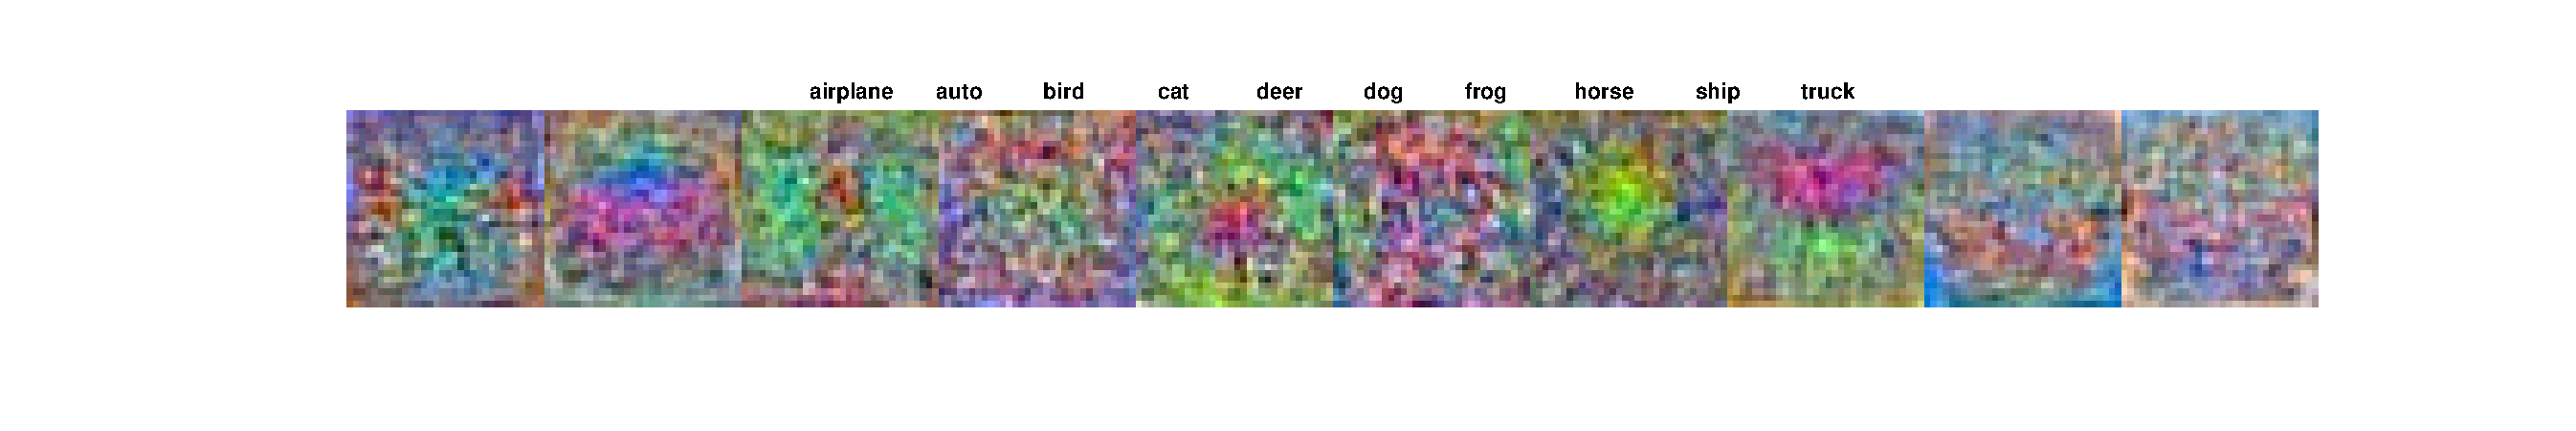
\includegraphics[scale=0.25]{figs/WeightMatrix_1}
  \caption{Learnt weight vectors for each class}
\label{sf:12}
\end{subfigure}

\caption{\texttt{lambda} = 0, \texttt{n\_epochs} = 40, \texttt{n\_batch} = 100, \texttt{eta} = 0.1}
\label{sf:1}

\end{figure}


% PS 2
\begin{figure}[h]
\centering

\begin{subfigure}{0.5\textwidth}
\centering
  \includegraphics[scale=0.47]{figs/Loss_2}
  \caption{Loss curve (Valdiation and Training sets)}
\label{sf:21}
\end{subfigure}

\begin{subfigure}{0.5\textwidth}
  \centering
  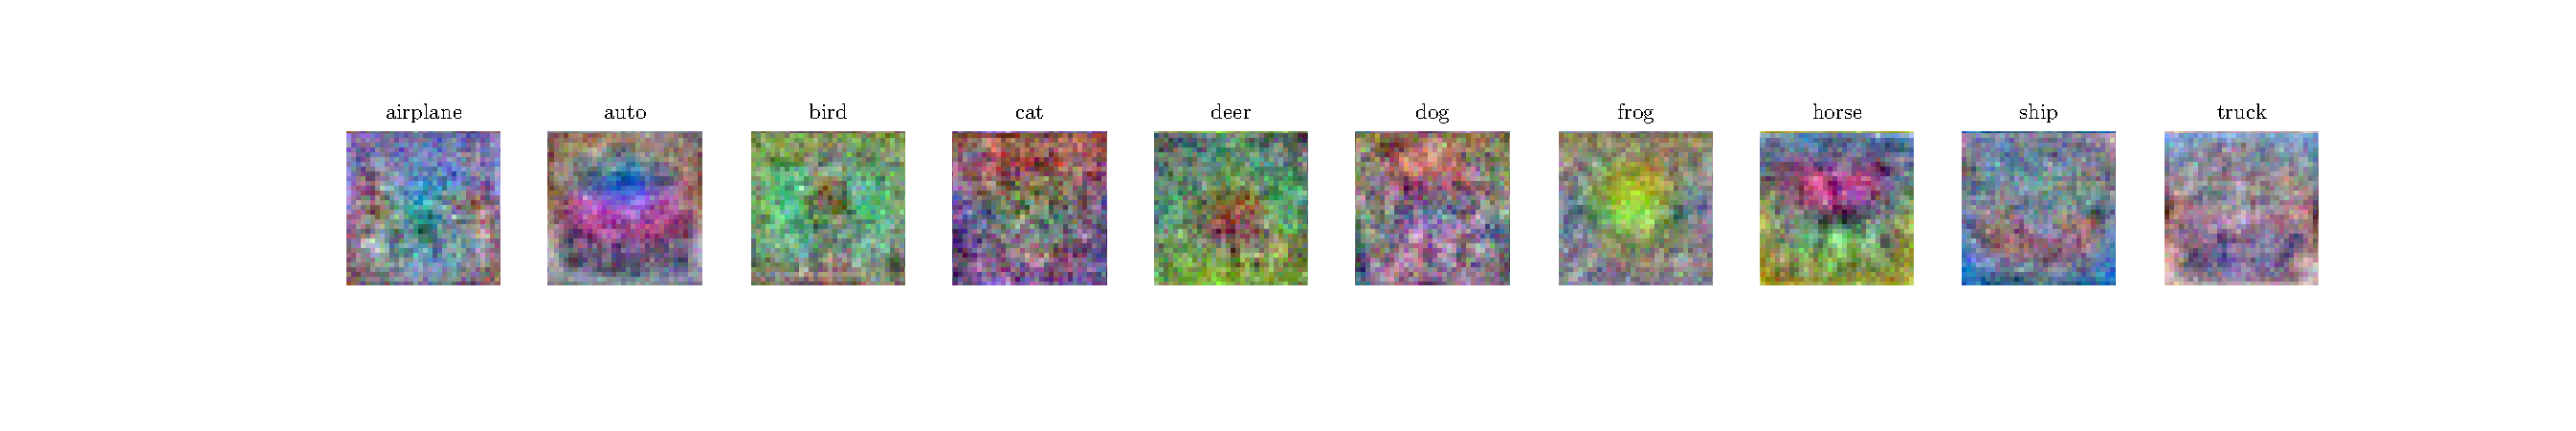
\includegraphics[scale=0.25]{figs/WeightMatrix_2}
  \caption{Learnt weight vectors for each class}
\label{sf:22}
\end{subfigure}

  \caption{\texttt{lambda} = 0, \texttt{n\_epochs} = 40, \texttt{n\_batch} = 100, \texttt{eta} = 0.01}
\label{sf:2}

\end{figure}

% PS 3
\begin{figure}[h]
\centering

\begin{subfigure}{0.5\textwidth}
  \centering
  \includegraphics[scale=0.47]{figs/Loss_3}
  \caption{Loss curve (Valdiation and Training sets)}
\label{sf:31}
\end{subfigure}

\begin{subfigure}{0.5\textwidth}
  \centering
  \includegraphics[scale=0.25]{figs/WeightMatrix_3}
  \caption{Learnt weight vectors for each class}
\label{sf:32}
\end{subfigure}

  \caption{\texttt{lambda} = 0.1, \texttt{n\_epochs} = 40, \texttt{n\_batch} = 100, \texttt{eta} = 0.01}
\label{sf:3}

\end{figure}

% PS 4
\begin{figure}[h]
 \centering

\begin{subfigure}{0.5\textwidth}
  \centering
  \includegraphics[scale=0.47]{figs/Loss_4}
  \caption{Loss curve (Valdiation and Training sets)}
\label{sf:41}
\end{subfigure}

\begin{subfigure}{0.5\textwidth}
  \centering
  \includegraphics[scale=0.25]{figs/WeightMatrix_4}
  \caption{Learnt weight vectors for each class}
\label{sf:42}
\end{subfigure}

  \caption{\texttt{lambda} = 1, \texttt{n\_epochs} = 40, \texttt{n\_batch} = 100, \texttt{eta} = 0.01}
\label{sf:4}

\end{figure}

\subsection{Discussion}

In Fig. \ref{sf:1} we observe that the cost curve is very noisy. This is mainly due to the too high learning rate value, which prevents the gradient descent algorithm to converge to a local minima. Thus, we should use a lower learning rate. Note, however, that too low learning rate will lead to slow convergence (time consuming). The accuracy obtained for this setting is of $22.55 \%$.

Fig. \ref{sf:2} illustrates the best result obtained from this four settings with an accuracy of $36.65 \%$. This has obtained repeating exactly the same parameter setting as before but decreasing the learning rate by a factor of 10.

Finally, Fig \ref{sf:3} and Fig \ref{sf:4} illustrate the effect of increasing the strength of the regularization term. In Fig \ref{sf:3} we note that the cost curves on both the validation and training sets have come close to each other. However the accuracy has decreased to $33.37 \%$. A reason for this might be that we are underfitting, that is we are trying to fit a too simplistic model. In the last figure we observe that the cost evaluation in the validation and training set is almost identical, but accuracy is now $21.92 \%$. From this we learn that while having similar loss in the training and validation set might be an indicator of not-overfitting, it does not necessarily mean that we are performing better. In particular, we can underfit!


\section{Exercise 2} \label{sec:2}

In this exercise, we will first try to optimize the results obtained in the first exercise. Next, I will implement the same network but with the SVM multi-class loss.

\subsection{Optimization of Exercise 1}

I have tried the following optimization methods:

\begin{itemize}
\item[1.] Permute order of samples
\item[2.] Center the data
\item[3.] Increase training set (decrease validation set)
\item[4.] Decrease factor for the learning rate
\item[5.] Add noise to training samples
\item[6.] Change batch size
\end{itemize}


Some of the listed methods were proven to increase the performance. However, specific combination of all of those had to be obtained experimentally. \\


In this regard, I took the parameter setting that performed the best in exercise 1, that is \texttt{lambda} = 0, \texttt{n\_epochs} = 40, \texttt{n\_batch} = 100, \texttt{eta} = 0.01, and tried to boost its performance.\\


A very simple yet powerfull improvement is to use Method 1, i.e. randomize the order of the data samples for each epoch. Doing so, we avoid using the exact same batches in the same exact order at each epoch and thus improve our chances of better generalization. With this, we achieve an accuracy of 38.08 \%. \\

Next, we center all the sets using the mean of the training set (Method 2). This simple change leads to an increase of the accuracy up to 39.48 \%.\\

To improve the generalization a very intuitive approach is to increase the size of the training set (Method 3). In this regard, we use 19000 samples for the training set, leaving just 1000 for the validation set. This change leads to an accuracy of 40.23 \%.  \\

After some trial and error, I decided to keep the learning rate constant. \\%Furthermore, decreasing the learning rate at each epoch by a factor of $0.99$ showed better results, reaching an accuracy of 40.23 \% on the test data. \\

Next, I tried Method 5, i.e. adding noise to the training samples, since it has been reported in the literature \cite{an1996effects} to improve the generalization. Adding zero-mean noise with standard deviation of $0.001$ showed as slight increase up to 40.32 \% accuracy. However, due to randomness this result might oscilate.\\


Finally, I trained 10 networks with this optimizations and combined them to obtain an ensembler of networks. The accuracy was increased up to 40.61 \%. \\


Ensemble method

\subsection{SVM multi-class loss}

%\begin{figure}[h]
%\center
%\includegraphics[scale=0.52]{figs/imgproc}
%\caption{The left image, shows the input frame with the artificially added occlusions (cyan filled rectangles). The right image illustrates the filtered $k$:th frame, i.e. $I_B(k)$, which shows likely regions for the ball highlighted in white. This particular result is for frame $k = 315$.}
%\label{fig:s}
%\end{figure}

%\begin{figure}[H]
%\centering
%\begin{minipage}{0.3\textwidth}
%{ \textbf{kalman\_filter} ($\mu_{k-1}, \Sigma_{k-1}, z_k$)}\\
%\indent ~ \textit{Step 1: Prediction}
%\begin{algorithmic}
%\State $\overline{\mu}_k \gets A \mu_{k-1}$
%\State $\overline{\Sigma}_k \gets A \Sigma_{k-1} A^T + R_k$
%\end{algorithmic}
%\break
%~ \textit{Step 2: Update}
%\begin{algorithmic}
%\State $K_k \gets \overline{\Sigma}_kC^T(C \overline{\Sigma}_kC^T+Q_k)^{-1}$
%\State $\mu_k \gets \overline{\mu}_k+K_k(z_k - C\overline{\mu}_k)$ \\
% $\Sigma_k \gets \overline{\Sigma}_k - K_kC\overline{\Sigma}_k$
%\end{algorithmic}
%~  \noindent \textbf{return} $\mu_k, \Sigma_k$

%\end{minipage}
%\caption{Kalman Filter Algorithm}
%\label{algo:1}
%\end{figure}

% This is how you define a table: the [!hbt] means that LaTeX is forced (by the !) to place the table exactly here (by h), or if that doesnt work because of a pagebreak or so, it tries to place the table to the bottom of the page (by b) or the top (by t).
%	\begin{table}[!hbt]
%		% Center the table
%		\begin{center}
%		% Title of the table
%		\caption{Simulation Parameters}
%		\label{tab:simParameters}
%		% Table itself: here we have two columns which are centered and have lines to the left, right and in the middle: |c|c|
%		\begin{tabular}{|c|c|}
%			% To create a horizontal line, type \hline
%			\hline
%			% To end a column type &
%			% For a linebreak type \\
%			Information message length & $k=16000$ bit \\
%			\hline
%			Radio segment size & $b=160$ bit \\
%			\hline
%			Rate of component codes & $R_{cc}=1/3$\\
%			\hline
%			Polynomial of component encoders & $[1 , 33/37 , 25/37]_8$\\
%			\hline
%		\end{tabular}
%		\end{center}
%	\end{table}

	% If you have questions about how to write mathematical formulas in LaTeX, please read a LaTeX book or the 'Not So Short Introduction to LaTeX': tobi.oetiker.ch/lshort/lshort.pdf

%%%%%%%%%%%%%%%%%%%%%%%%%%%%%%%%%%%%%%%%%%%%%%%%%%%%%%%%%%%%%%%%%%%%%%%%%%
%%%%%%%%%%%%%%%%%%%%%%%%%%%%%%%%%%%%%%%%%%%%%%%%%%%%%%%%%%%%%%%%%%%%%%%%%%


%MSE PF = 1.034961e+02
%MSE KF = 4.169997e+01
%MSE combined = 9.995835e+01
%---
%MSE PF = 3.547435e+03
%MSE KF = 4.169997e+01
%MSE combined = 3.568715e+03



%\subsection{Constant Velocity model}
%\subsection{Constant Acceleration model}

%MSE PF = 8.983220e+03
%MSE KF = 4.807877e+01
%MSE combined = 9.003513e+03

%\begin{figure*}[h]
%\centering
%\begin{subfigure}{\textwidth}
%  \includegraphics[scale=0.4]{figs/mse_vel_good}
%  \caption{Squared error for each frame for a constant velocity model. Kalman Filter turned out to perform at best}
%\label{sf:1}
%\end{subfigure}

%\begin{subfigure}{\textwidth}
%  \includegraphics[scale=0.4]{figs/mse_acc_good}
%  \caption{Squared error for each frame for a constant acceleration model. Kalman Filter turned out to perform at best}
%\label{sf:2}
%\end{subfigure}

%\begin{subfigure}{\textwidth}
%  \includegraphics[scale=0.4]{figs/mse_acc_bad}
%  \caption{In this execution, we observe the phenomena of particle deprivation. This is seen in the high values of squared error for some frame intervals, which ultimately correspond to instances when the ball is occluded and hence its track is lost by the particle cloud.}
%\label{sf:3}
%\end{subfigure}


%\begin{subfigure}{\textwidth}
% \centering
%  \includegraphics[scale=0.4]{figs/mseplot1}
%  \caption{MSE for each frame for Case 2, where we had Particle Deprivation.}
%\end{subfigure}

%\caption{MSE for each frame for different executions of the 15 second frame sequence. Peaky values are usually associated with frame intervals where the ball is occluded.}
%\label{fig:mseplot}
%\end{figure*}


%%%%%%%%%%%%%%%%%%%%%%%%%%%%%%%%%%%%%%%%%%%%%%%%%%%%%%%%%%%%%%%%%%%%%%%%%%
%%%%%%%%%%%%%%%%%%%%%%%%%%%%%%%%%%%%%%%%%%%%%%%%%%%%%%%%%%%%%%%%%%%%%%%%%%

%The code for this project can be found in this \href{https://github.com/lucasrodes/el2320-project}{link}.
%%%%%%%%%%%%%%%%%%%%%%%%%%%%%%%%%%%%%%%%%%%%%%%%%%%%%%%%%%%%%%%%%%%%%%%%%%
%%%%%%%%%%%%%%%%%%%%%%%%%%%%%%%%%%%%%%%%%%%%%%%%%%%%%%%%%%%%%%%%%%%%%%%%%%
%\section*{Appendix} \label{sec:appendix}
% Now we need a bibliography:

\bibliographystyle{unsrt}
\bibliography{refs}
% Your document ends here!
\end{document}